% *** Authors should verify (and, if needed, correct) their LaTeX system  ***
% *** with the testflow diagnostic prior to trusting their LaTeX platform ***
% *** with production work. IEEE's font choices and paper sizes can       ***
% *** trigger bugs that do not appear when using other class files.       ***                          ***
% The testflow support page is at:
% http://www.michaelshell.org/tex/testflow/



\documentclass[conference,compsoc]{IEEEtran}
% Some/most Computer Society conferences require the compsoc mode option,
% but others may want the standard conference format.
%
% If IEEEtran.cls has not been installed into the LaTeX system files,
% manually specify the path to it like:
% \documentclass[conference,compsoc]{../sty/IEEEtran}
%\usepackage{hyperref}
\usepackage{graphicx}



% Some very useful LaTeX packages include:
% (uncomment the ones you want to load)


% *** MISC UTILITY PACKAGES ***
%
%\usepackage{ifpdf}
% Heiko Oberdiek's ifpdf.sty is very useful if you need conditional
% compilation based on whether the output is pdf or dvi.
% usage:
% \ifpdf
%   % pdf code
% \else
%   % dvi code
% \fi
% The latest version of ifpdf.sty can be obtained from:
% http://www.ctan.org/tex-archive/macros/latex/contrib/oberdiek/
% Also, note that IEEEtran.cls V1.7 and later provides a builtin
% \ifCLASSINFOpdf conditional that works the same way.
% When switching from latex to pdflatex and vice-versa, the compiler may
% have to be run twice to clear warning/error messages.






% *** CITATION PACKAGES ***
%
\ifCLASSOPTIONcompsoc
  % IEEE Computer Society needs nocompress option
  % requires cite.sty v4.0 or later (November 2003)
  \usepackage[nocompress]{cite}
\else
  % normal IEEE
  \usepackage{cite}
\fi
% cite.sty was written by Donald Arseneau
% V1.6 and later of IEEEtran pre-defines the format of the cite.sty package
% \cite{} output to follow that of IEEE. Loading the cite package will
% result in citation numbers being automatically sorted and properly
% "compressed/ranged". e.g., [1], [9], [2], [7], [5], [6] without using
% cite.sty will become [1], [2], [5]--[7], [9] using cite.sty. cite.sty's
% \cite will automatically add leading space, if needed. Use cite.sty's
% noadjust option (cite.sty V3.8 and later) if you want to turn this off
% such as if a citation ever needs to be enclosed in parenthesis.
% cite.sty is already installed on most LaTeX systems. Be sure and use
% version 5.0 (2009-03-20) and later if using hyperref.sty.
% The latest version can be obtained at:
% http://www.ctan.org/tex-archive/macros/latex/contrib/cite/
% The documentation is contained in the cite.sty file itself.
%
% Note that some packages require special options to format as the Computer
% Society requires. In particular, Computer Society  papers do not use
% compressed citation ranges as is done in typical IEEE papers
% (e.g., [1]-[4]). Instead, they list every citation separately in order
% (e.g., [1], [2], [3], [4]). To get the latter we need to load the cite
% package with the nocompress option which is supported by cite.sty v4.0
% and later.





% *** GRAPHICS RELATED PACKAGES ***
%
\ifCLASSINFOpdf
  % \usepackage[pdftex]{graphicx}
  % declare the path(s) where your graphic files are
  % \graphicspath{{../pdf/}{../jpeg/}}
  % and their extensions so you won't have to specify these with
  % every instance of \includegraphics
  % \DeclareGraphicsExtensions{.pdf,.jpeg,.png}
\else
  % or other class option (dvipsone, dvipdf, if not using dvips). graphicx
  % will default to the driver specified in the system graphics.cfg if no
  % driver is specified.
  % \usepackage[dvips]{graphicx}
  % declare the path(s) where your graphic files are
  % \graphicspath{{../eps/}}
  % and their extensions so you won't have to specify these with
  % every instance of \includegraphics
  % \DeclareGraphicsExtensions{.eps}
\fi
% graphicx was written by David Carlisle and Sebastian Rahtz. It is
% required if you want graphics, photos, etc. graphicx.sty is already
% installed on most LaTeX systems. The latest version and documentation
% can be obtained at: 
% http://www.ctan.org/tex-archive/macros/latex/required/graphics/
% Another good source of documentation is "Using Imported Graphics in
% LaTeX2e" by Keith Reckdahl which can be found at:
% http://www.ctan.org/tex-archive/info/epslatex/
%
% latex, and pdflatex in dvi mode, support graphics in encapsulated
% postscript (.eps) format. pdflatex in pdf mode supports graphics
% in .pdf, .jpeg, .png and .mps (metapost) formats. Users should ensure
% that all non-photo figures use a vector format (.eps, .pdf, .mps) and
% not a bitmapped formats (.jpeg, .png). IEEE frowns on bitmapped formats
% which can result in "jaggedy"/blurry rendering of lines and letters as
% well as large increases in file sizes.
%
% You can find documentation about the pdfTeX application at:
% http://www.tug.org/applications/pdftex





% *** MATH PACKAGES ***
%
%\usepackage[cmex10]{amsmath}
% A popular package from the American Mathematical Society that provides
% many useful and powerful commands for dealing with mathematics. If using
% it, be sure to load this package with the cmex10 option to ensure that
% only type 1 fonts will utilized at all point sizes. Without this option,
% it is possible that some math symbols, particularly those within
% footnotes, will be rendered in bitmap form which will result in a
% document that can not be IEEE Xplore compliant!
%
% Also, note that the amsmath package sets \interdisplaylinepenalty to 10000
% thus preventing page breaks from occurring within multiline equations. Use:
%\interdisplaylinepenalty=2500
% after loading amsmath to restore such page breaks as IEEEtran.cls normally
% does. amsmath.sty is already installed on most LaTeX systems. The latest
% version and documentation can be obtained at:
% http://www.ctan.org/tex-archive/macros/latex/required/amslatex/math/





% *** SPECIALIZED LIST PACKAGES ***
%
%\usepackage{algorithmic}
% algorithmic.sty was written by Peter Williams and Rogerio Brito.
% This package provides an algorithmic environment fo describing algorithms.
% You can use the algorithmic environment in-text or within a figure
% environment to provide for a floating algorithm. Do NOT use the algorithm
% floating environment provided by algorithm.sty (by the same authors) or
% algorithm2e.sty (by Christophe Fiorio) as IEEE does not use dedicated
% algorithm float types and packages that provide these will not provide
% correct IEEE style captions. The latest version and documentation of
% algorithmic.sty can be obtained at:
% http://www.ctan.org/tex-archive/macros/latex/contrib/algorithms/
% There is also a support site at:
% http://algorithms.berlios.de/index.html
% Also of interest may be the (relatively newer and more customizable)
% algorithmicx.sty package by Szasz Janos:
% http://www.ctan.org/tex-archive/macros/latex/contrib/algorithmicx/




% *** ALIGNMENT PACKAGES ***
%
%\usepackage{array}
% Frank Mittelbach's and David Carlisle's array.sty patches and improves
% the standard LaTeX2e array and tabular environments to provide better
% appearance and additional user controls. As the default LaTeX2e table
% generation code is lacking to the point of almost being broken with
% respect to the quality of the end results, all users are strongly
% advised to use an enhanced (at the very least that provided by array.sty)
% set of table tools. array.sty is already installed on most systems. The
% latest version and documentation can be obtained at:
% http://www.ctan.org/tex-archive/macros/latex/required/tools/


% IEEEtran contains the IEEEeqnarray family of commands that can be used to
% generate multiline equations as well as matrices, tables, etc., of high
% quality.




% *** SUBFIGURE PACKAGES ***
%\ifCLASSOPTIONcompsoc
%  \usepackage[caption=false,font=footnotesize,labelfont=sf,textfont=sf]{subfig}
%\else
%  \usepackage[caption=false,font=footnotesize]{subfig}
%\fi
% subfig.sty, written by Steven Douglas Cochran, is the modern replacement
% for subfigure.sty, the latter of which is no longer maintained and is
% incompatible with some LaTeX packages including fixltx2e. However,
% subfig.sty requires and automatically loads Axel Sommerfeldt's caption.sty
% which will override IEEEtran.cls' handling of captions and this will result
% in non-IEEE style figure/table captions. To prevent this problem, be sure
% and invoke subfig.sty's "caption=false" package option (available since
% subfig.sty version 1.3, 2005/06/28) as this is will preserve IEEEtran.cls
% handling of captions.
% Note that the Computer Society format requires a sans serif font rather
% than the serif font used in traditional IEEE formatting and thus the need
% to invoke different subfig.sty package options depending on whether
% compsoc mode has been enabled.
%
% The latest version and documentation of subfig.sty can be obtained at:
% http://www.ctan.org/tex-archive/macros/latex/contrib/subfig/




% *** FLOAT PACKAGES ***
%
%\usepackage{fixltx2e}
% fixltx2e, the successor to the earlier fix2col.sty, was written by
% Frank Mittelbach and David Carlisle. This package corrects a few problems
% in the LaTeX2e kernel, the most notable of which is that in current
% LaTeX2e releases, the ordering of single and double column floats is not
% guaranteed to be preserved. Thus, an unpatched LaTeX2e can allow a
% single column figure to be placed prior to an earlier double column
% figure. The latest version and documentation can be found at:
% http://www.ctan.org/tex-archive/macros/latex/base/


%\usepackage{stfloats}
% stfloats.sty was written by Sigitas Tolusis. This package gives LaTeX2e
% the ability to do double column floats at the bottom of the page as well
% as the top. (e.g., "\begin{figure*}[!b]" is not normally possible in
% LaTeX2e). It also provides a command:
%\fnbelowfloat
% to enable the placement of footnotes below bottom floats (the standard
% LaTeX2e kernel puts them above bottom floats). This is an invasive package
% which rewrites many portions of the LaTeX2e float routines. It may not work
% with other packages that modify the LaTeX2e float routines. The latest
% version and documentation can be obtained at:
% http://www.ctan.org/tex-archive/macros/latex/contrib/sttools/
% Do not use the stfloats baselinefloat ability as IEEE does not allow
% \baselineskip to stretch. Authors submitting work to the IEEE should note
% that IEEE rarely uses double column equations and that authors should try
% to avoid such use. Do not be tempted to use the cuted.sty or midfloat.sty
% packages (also by Sigitas Tolusis) as IEEE does not format its papers in
% such ways.
% Do not attempt to use stfloats with fixltx2e as they are incompatible.
% Instead, use Morten Hogholm'a dblfloatfix which combines the features
% of both fixltx2e and stfloats:
%
% \usepackage{dblfloatfix}
% The latest version can be found at:
% http://www.ctan.org/tex-archive/macros/latex/contrib/dblfloatfix/




% *** PDF, URL AND HYPERLINK PACKAGES ***
%
%\usepackage{url}
% url.sty was written by Donald Arseneau. It provides better support for
% handling and breaking URLs. url.sty is already installed on most LaTeX
% systems. The latest version and documentation can be obtained at:
% http://www.ctan.org/tex-archive/macros/latex/contrib/url/
% Basically, \url{my_url_here}.




% *** Do not adjust lengths that control margins, column widths, etc. ***
% *** Do not use packages that alter fonts (such as pslatex).         ***
% There should be no need to do such things with IEEEtran.cls V1.6 and later.
% (Unless specifically asked to do so by the journal or conference you plan
% to submit to, of course. )


% correct bad hyphenation here
\hyphenation{op-tical net-works semi-conduc-tor}


\begin{document}

%
% paper title
% Titles are generally capitalized except for words such as a, an, and, as,
% at, but, by, for, in, nor, of, on, or, the, to and up, which are usually
% not capitalized unless they are the first or last word of the title.
% Linebreaks \\ can be used within to get better formatting as desired.
% Do not put math or special symbols in the title.
\title{Procedural Content generation: Adaptive dungeon generator}


% author names and affiliations
% use a multiple column layout for up to three different
% affiliations
\author{
\IEEEauthorblockN{Mikkel Stolborg, Mats Stenhaug}
\IEEEauthorblockA{Games and Technology\\
IT-University of Copenhagen\\
Copenhagen, Denmark\\
Email: msto@itu.dk}
% Template for adding other people
%\and
%\IEEEauthorblockN{Homer Simpson}
%\IEEEauthorblockA{Twentieth Century Fox\\
%Springfield, USA\\
%Email: homer@thesimpsons.com}
%\and
%\IEEEauthorblockN{James Kirk\\ and Montgomery Scott}
%\IEEEauthorblockA{Starfleet Academy\\
%San Francisco, California 96678-2391\\
%Telephone: (800) 555--1212\\
%Fax: (888) 555--1212}
}

% conference papers do not typically use \thanks and this command
% is locked out in conference mode. If really needed, such as for
% the acknowledgment of grants, issue a \IEEEoverridecommandlockouts
% after \documentclass

% for over three affiliations, or if they all won't fit within the width
% of the page (and note that there is less available width in this regard for
% compsoc conferences compared to traditional conferences), use this
% alternative format:
% 
%\author{\IEEEauthorblockN{Michael Shell\IEEEauthorrefmark{1},
%Homer Simpson\IEEEauthorrefmark{2},
%James Kirk\IEEEauthorrefmark{3}, 
%Montgomery Scott\IEEEauthorrefmark{3} and
%Eldon Tyrell\IEEEauthorrefmark{4}}
%\IEEEauthorblockA{\IEEEauthorrefmark{1}School of Electrical and Computer Engineering\\
%Georgia Institute of Technology,
%Atlanta, Georgia 30332--0250\\ Email: see http://www.michaelshell.org/contact.html}
%\IEEEauthorblockA{\IEEEauthorrefmark{2}Twentieth Century Fox, Springfield, USA\\
%Email: homer@thesimpsons.com}
%\IEEEauthorblockA{\IEEEauthorrefmark{3}Starfleet Academy, San Francisco, California 96678-2391\\
%Telephone: (800) 555--1212, Fax: (888) 555--1212}
%\IEEEauthorblockA{\IEEEauthorrefmark{4}Tyrell Inc., 123 Replicant Street, Los Angeles, California 90210--4321}}




% use for special paper notices
%\IEEEspecialpapernotice{(Invited Paper)}




% make the title area
\maketitle

% As a general rule, do not put math, special symbols or citations
% in the abstract
\begin{abstract}
The abstract goes here.
\end{abstract}

% no keywords




% For peer review papers, you can put extra information on the cover
% page as needed:
% \ifCLASSOPTIONpeerreview
% \begin{center} \bfseries EDICS Category: 3-BBND \end{center}
% \fi
%
% For peerreview papers, this IEEEtran command inserts a page break and
% creates the second title. It will be ignored for other modes.
\IEEEpeerreviewmaketitle



\section{Introduction}
% no \IEEEPARstart
We wanted to make a board game dungeon map creator in this project. Having rooms, doors, items and interactables being procedurally generated on the fly, as we journeyed through the dungeon. 
Our idea was to create this in a way that utilized PCG in some sort of manner that would make the user feel like it was part of a "story" in some sense, or that everything had some sort of connection. 

This also meant that we wanted to give the user some sense of choice. Whether it was to possible directions to venture, or to have some sort of interactive decision-point where the user would have to set the scene for how the next parts of the dungeon would be generated. A simple example we came up with was to have the player choose whether he or she felt adventurous or not. Using this information in order to toggle if the dungeon should have a lot of bends and be made very spread, or if it should be more linear and maybe shorter.

Our problem statement was formed to be something like this:
\begin{itemize}
\item[-] \textit{Procedurally generate a dungeon and it's contents in real-time, as the player explores what is already generated. Making points along the way where enemies, treasure or other points of interest can be found and interacted with.}
\end{itemize}

Initially we wanted to create something really big. Having the dungeon implement some sort of history. So say that if the player were to kill an enemy, the game would then know that that type of creature would act more hostile the next time the player would encounter them. And on the other side, if the player were to help that "enemy", maybe it would become a friend instead?

If we wanted to implement this type of history and decision making into the generator, we would also have to find some sort of way to generate these options and decisions as the player progress through the dungeon.

In this document, we will elaborate and discuss on the implementations we made, how we narrowed down our scope in accordance with the supervisor, and how we came to the conclusions that we did.
	
\section{Background}
Procedural content generation for maps and dungeon creation has been used a multitude of time over the years. So what we wanted to do for our project, in order to hopefully make it stand out, was to try to implement the element of decisions and history. By having close to everything being generated as you go along, would make it possible to generate a huge amount of different scenarios, maps and game plays. Technically speaking, every play-through could be different. 
Our goals and wants for this project was initially set very high, as we wanted to have the opportunity to implement as much of our vision as possible. How much we can implement, and how the scope may be narrowed down, remains to be seen.

There are plenty of concepts, ideas and pre-made generators out there, and it can be quite informative to look into those, read about how other people have made their solutions, and get ideas to how we can improve and make our project as good as we are able.

\begin{figure}[h]
	\graphicspath{{figures/}}
	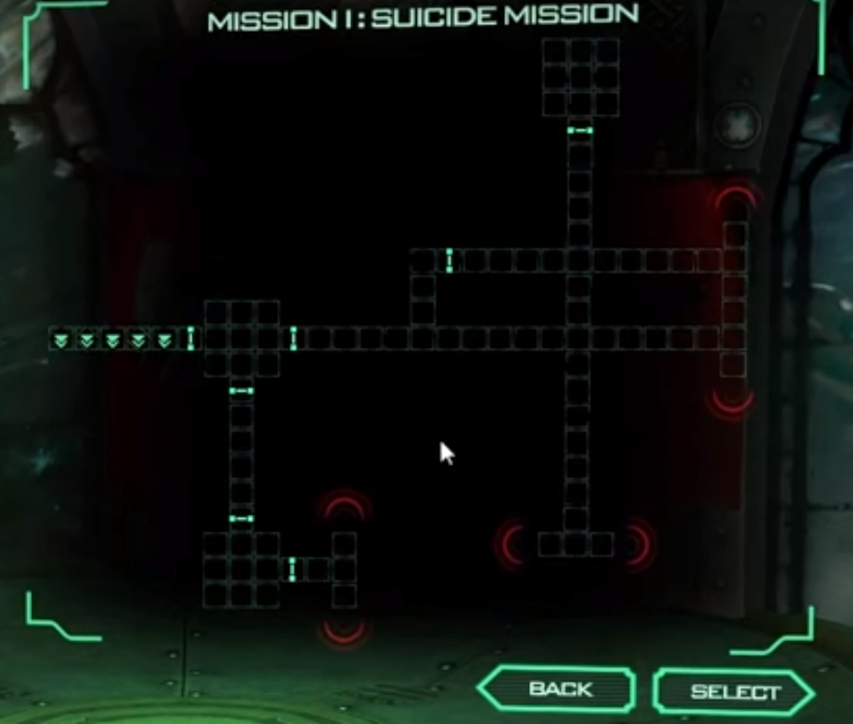
\includegraphics[width = \columnwidth ]{SpacehulkMap.png}
	\caption{Layout of a mission map for the game Space Hulk.}
	\label{fig:spacehulk}
\end{figure}

In figure \ref{fig:spacehulk} you can see a map layout of a level of the digital version of the game Space Hulk\cite{SpaceHulkvid}. This was used as initial reference for our idea, as it is a digital representation of a board game. It is a very simple layout, but it has the key elements that we wanted as well. Rooms, doors and hallways.
The video game is directly based on the board game version with the same name\cite{SpaceHulkBoard}, and as such is related to the idea we had about generating a board game map through a piece system in a digital tool and context. 

Further games generates dungeon structures, an example being the game from Blizzard North, Diablo II\cite{Diablo2}. It generates the levels the player traverses on game creation. Though the layout is not fuelled by player actions, its generation of levels provides a greater replayability. 

When our generator is complete, we are hoping to use some smart algorithms, like A-Star, in order to validate if our dungeons are viable. We will have to use this in-game as we generate as well, if we hope to create our maps "on the go" since we want the room placements to be dependent on how the player interacts with the world we create for them.

We believe that making this dungeon generator/exploration game will be an interesting project, as we will get to put our minds together to come up with what we hope will be great ideas as to how we can create fun and interesting dungeons. 

\section{Game Design}
The core mechanics of the game are purely based on PCG. Without it, the game would simply not be possible. Of course, we could always create dungeons using manual design, and a paper-to-code approach. But since we want to make a game that is purely based on PCG, we need to create every algorithm from scratch, and we have to make calculated design approaches in order to make the algorithms as we want them.

Our first and foremost milestone, is to come up with a way of creating the dungeon in such a fashion that we can validate how good it is, and from there, make it so that we can add more features into it, like creating objects, enemies and other interactables. 

Our approach to generating the dungeon, rooms and content in real-time, will be to first create a dungeon generator that will instantly create the entire dungeon in one go. That means all the rooms, doors and hallways. This means that we will have to come up with a clever way of making a complete layout of the generated content. Making sure that the sizes of the rooms do not exceed the total size of the map, and to enable the dungeons to be generated in different sizes and shapes. Just because we initially want to be able to create a complete dungeon, doesn't mean we always want to create the same one, as that would not really constitute the sort of procedural content generation that we want. 
From there our task will be to break it down into pieces. Have only a single room be created from the start, and then expand on that room. Having one or more doors or ways to exit the room in different directions, and then generate new rooms that will be visible to the player.

Once we are able to generate a dungeon be creating new rooms and connecting them to the existing map, as the game is being played, the next step will be to have some form of content in the rooms.
The start point will, for the sake of simplicity and control, always be in the center of the first room that is created. But as we expand on our dungeon, we will need to have some sort of end condition. So what we will do is to implement an exit area. At first we thought about having the exit point be set from the start, and then create the rooms in the map so that they would eventually reach that point. But as we thought about it more and more, we realized that this was not how we wanted it. 

We wanted the players to explore as much as possible, without having to think about where the exact point of the exit were. So what we came up with, was to have the "adventure" scale. Basically what that means, is that the player gets the choice to select how "adventurous" he or she is feeling, and have that decision factor into the generation of the game space. If the player is feeling adventurous, the dungeons will be generated with rooms that spread more out, and that has more options of directions that are accessible. And going back to the end point; we believe the game would be more fun if the exit is generated suddenly, when you enter a new room that was previously unexplored. And when the exit would appear, would in some way be connected to how adventurous the player was.

With the ending condition now figured out, the thoughts on how we would generate other items in-game, like treasure, enemies, etc. arose. After brainstorming for quite some time, we came to the conclusion that these items and interactables should be dependent on the adventure-meter, but also be dependent on an element of luck and chance.
Creating rooms that were dead ends, could significantly increase the chance for an encounter of some sort to happen.

\section{Methods}
Our algorithm starts off by creating a board element, then having a room spawn in the center of said board. The center room, see figure \ref{fig:startroom}, will contain the starting point for the player, and will have 4 doors leading out of it in all possible movement directions, North, East, South and West.
After the board and starting room are initiated, the player object is generated and placed on the starting point. From here, all the elements that are now contained in the room will be drawn up on the screen and the player can now explore.

\begin{figure}[h]
	\graphicspath{{figures/}}
	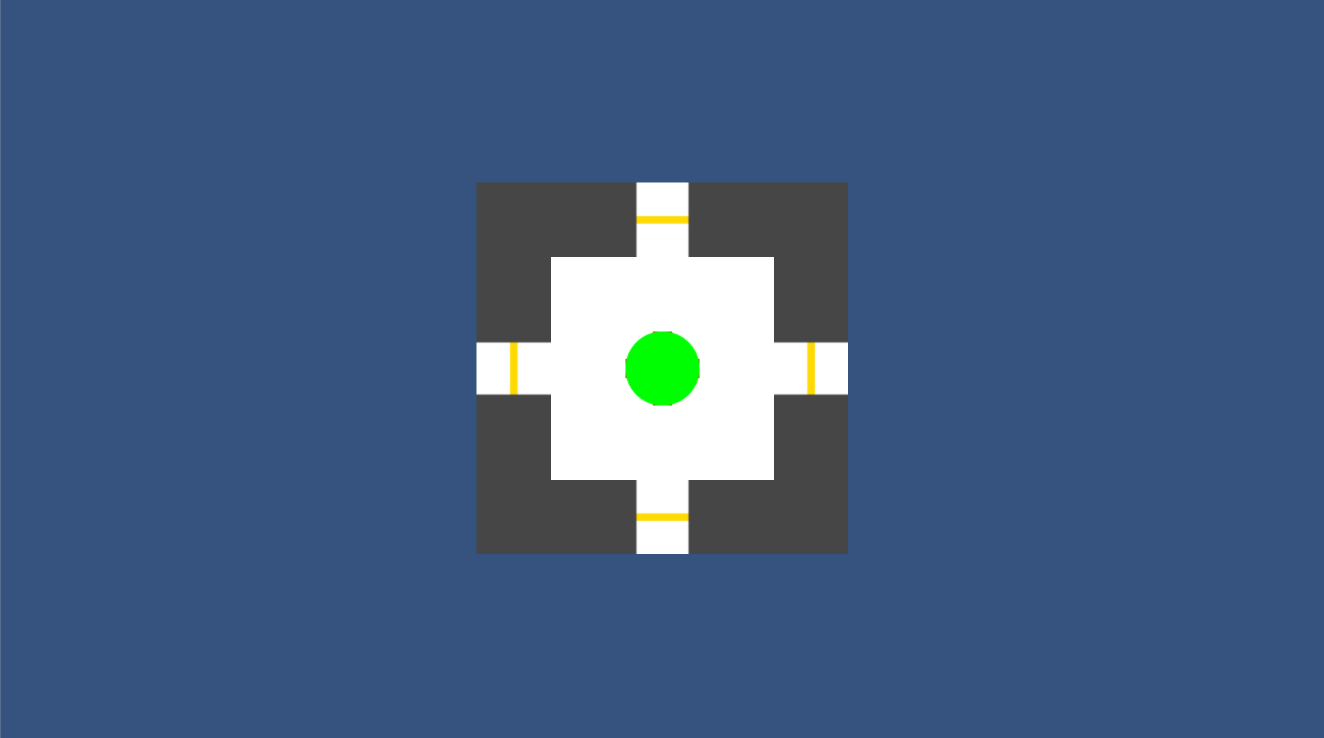
\includegraphics[width = \columnwidth ]{StartLayout.png}
	\caption{Initial dungeon layout. A center room with the player token and 4 doors leading out from it.}
	\label{fig:startroom}
\end{figure}

When the player walks through the first door (any of the initial 4 doors), the algorithm creates a new room in that direction. 
Since this is the first room that is generated, it will also contain an interactable spot where, if you walk on it, an option will appear on the screen that will allow the player to choose whether or not he or she wants the game to be adventurous or not. Interacting with the spot, known as the dialog interaction spot, allows for the game to get player feedback on their desire for how they want to play the game.

\begin{figure}[h]
	\graphicspath{{figures/}}
	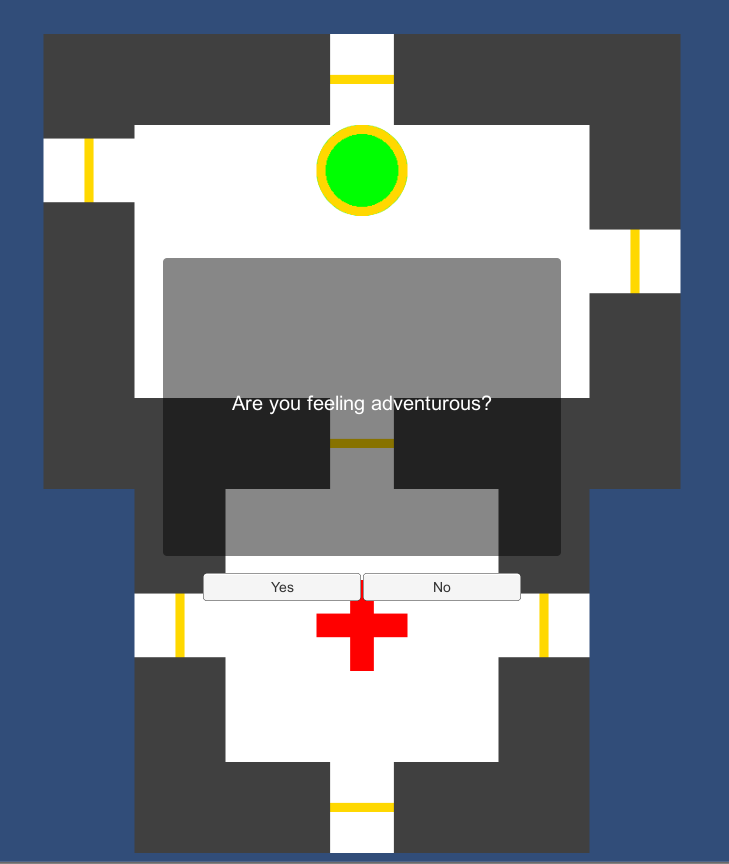
\includegraphics[width = \columnwidth ]{DialogSet.png}
	\caption{Dungeon with dialog interaction point placed. The Interaction point is represented by the yellow circle.}
	\label{fig:dialogset}
\end{figure}

The rooms have a chance of making from 0 to 3 doors. Number of doors spawned depend on the adventureness of the players as described in section \ref{sec:adven}.

\begin{figure}[h]
	\graphicspath{{figures/}}
	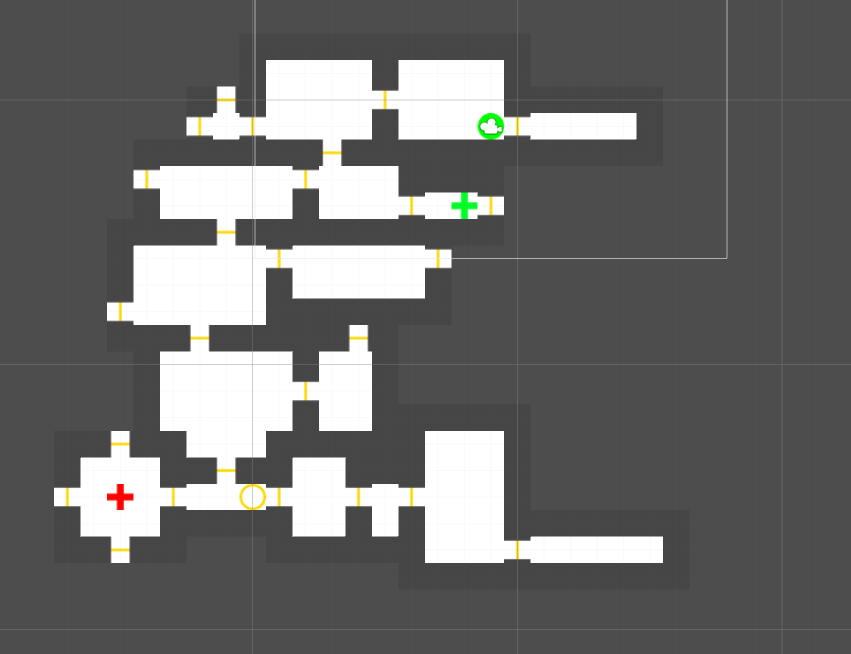
\includegraphics[width = \columnwidth ]{DungeonLayout.png}
	\caption{A partially explored dungeon with an exit spawned}
	\label{fig:dungparexit}
\end{figure}
Once you have explored a lot of the dungeon, the exit point will have an increasing chance of spawning. Even if it spawns, you can always avoid going on it, and keep exploring, if that is what you want. But once you enter the exit spot, the dungeon will reset and you will start a new dungeon adventure.
In figure \ref{fig:dungparexit} you can see an example of a partially explored dungeon with an exit spawned. As one can see there is still more dungeon to be explored, even though the exit has already been spawned.

\subsection{Adventureness of the player}
\label{sec:adven}
The adventureness of the player is set based on the interaction with the dialog interaction spot. It is more a stand-in for deeper gameplay interaction, and serves as a point where the algorithm can get a value which determines the players mindset when playing the game. 

The adventureness scale is used in several of the random algorithms to push the outcome towards the players wishes. A more adventurous player will have a higher adventureness score, whilst a lower score is awarded to less adventurous players.

The two most important uses are for when to generate the exit and the number of doors in a newly generated room. 
The exit placement chance is based on the adventureness of the player and how long the player has been playing, measured in terms of moves made.
The actual chance also uses a combined value of how much a player have moved, compared to the distance from the center of the map. This parameter, called advententurenessCalc is explained in more detail in section \ref{sec:adventCalc}. 
The final calculation used can be seen in equation \ref{eq:exit}.

\begin{equation}
\label{eq:exit}
chanceOfExit = \frac{1}{1 + e^{-\frac{Tc}{AS*AC*t+1}}}
\end{equation}

The terms used in equation \ref{eq:exit} are as follows. 

\textit{Tc} is the turn count of the game. It is a measure of how long time the game has passed.

\textit{AS} is the adventureness of the player and takes a value between 0 and 1. 

\textit{AC} is the advententurenessCalc, which is a calculated value explained in section \ref{sec:adventCalc}.

\textit{t} is a time scale factor.

The general gist of the function is that the longer the player spends in the game, the more of a chance there is to spawn the exit. The rest of the terms are there to prolong the game based on the players adventureness.

The number of doors created in a new room is a direct consequence of how adventurous the player is. There is always a chance for creating any number of doors, but the chance of more than one door is significantly increased based on the players adventureness.

\subsubsection{AdventurenessCalc scale value}
\label{sec:adventCalc}
The adventurenessCalc value is an attempt to gather information about the players mindset real-time throughout the game.
The value is calculated based on the how much the player moves around compared to how long the player has moved. The idea behind the value is that player who seek to explore more, will move around more than players we simply wishes to complete the level. 

\subsection{A-star distance measure algorithm}
\label{sec:astar}
In addition to our own algorithms, we use the A-star algorithms 

\section{Results}
\subsection{Did it work}
We weren't able to implement all the features that we wanted, which were described in the introduction and background. Our original idea was too out of scope, with much too many goals that would be unreachable given the time we had for our project. Even though not all we wanted to do, was completed, we were able to implement the most important features; having a dungeon being created in real-time, allowing the players to explore the dungeons as they see fit. Whether they are feeling adventurous, or just want to have a quick map and be done with it. 
By utilizing the A-Star algorithm, we were able to make the rooms get different "adventure"-values based on how far away from the start they are, how much the players have explored, and how adventurous they have been. The chance for a room to spawn more doors, and in turn, more opportunities and choices for the player, are also based on the adventure-meter and the A-Star. If you for instance are far away from the start (have explored quite a bit), the chance to walk into a dead end are increased.

The win condition is also based on how adventurous the player is. If they are feeling like exploring a huge dungeon, then the end-point will not spawn until the map "feels" like it has offered a lot of options and diversity.

\begin{figure}[h]
	\graphicspath{{figures/}}
	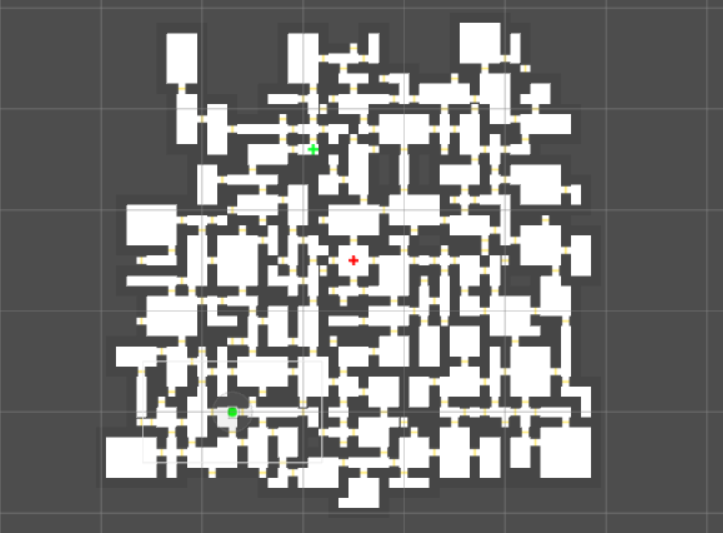
\includegraphics[width = \columnwidth ]{BigDungeon.png}
	\caption{Picture of a massive dungeon created by adventurous player}
	\label{fig:behavTree}
\end{figure}
\subsection{How well}
There were a lot of debugging required in order to create the dungeons as we wanted them to be created. Things took more time than we originally planned, which forced us to narrow down our scope, in accordance with our project supervisor. We still wanted to have multiple choices for the player, something that would give the feel of adventure and exploration. So by adding the option for the player to enable "adventure-mode", gave us the sensation of creating bigger and more diverse dungeons.
\begin{figure}[h]
	\graphicspath{{figures/}}
	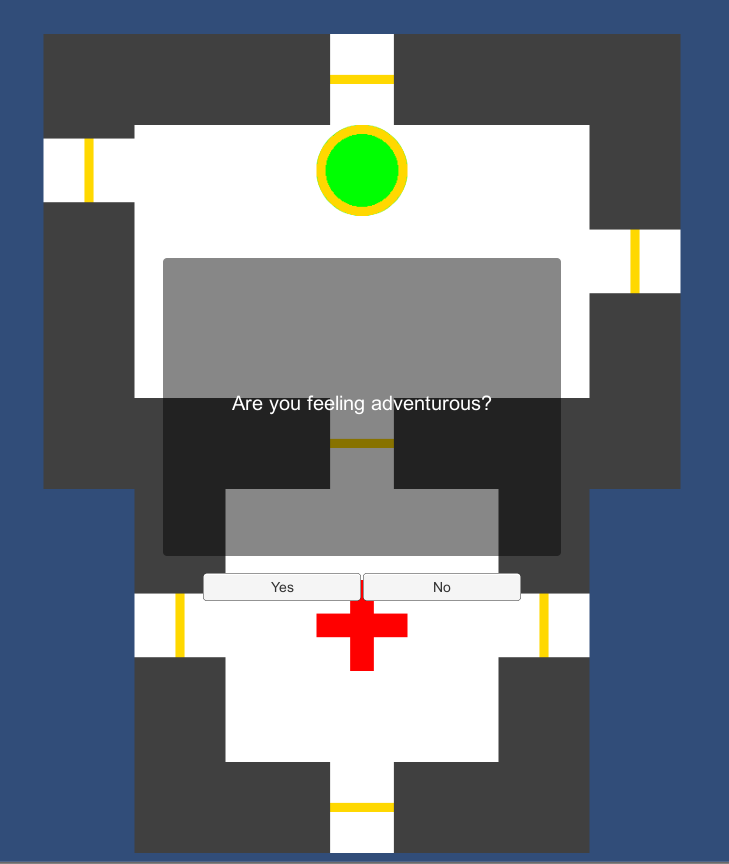
\includegraphics[width = \columnwidth ]{DialogSet.png}
	\caption{On this picture, you see the simple interface for selecting adventure mode or not.}
	\label{fig:behavTree}
\end{figure}
Some of the issues that came up during development were that the generator itself wasn't acting as we wanted it to. Rooms were created with doors that would lead nowhere or into a wall. So during development, we had to restructure and create new algorithms for the generator to work. This took a lot of time. Too much time in fact. Because of us having to remake the generators so much, we decided to make a completely new one from scratch, that took the best features we knew worked, and utilized them in a new way. This turned out to be a great choice, which allowed us to fix many of those bugs we had with the doors and what not.

Our finished product turned out to be very up to par with the feel we wanted to go for. We only use a simple interface, and graphics, although simple, are there only to let the player see which possibilities that are presented. 
A fully generated dungeon will be quite huge, and as you can see from the next figure, the player will have had to do a lot of choices in order to make it. 

\begin{figure}[h]
	\graphicspath{{figures/}}
	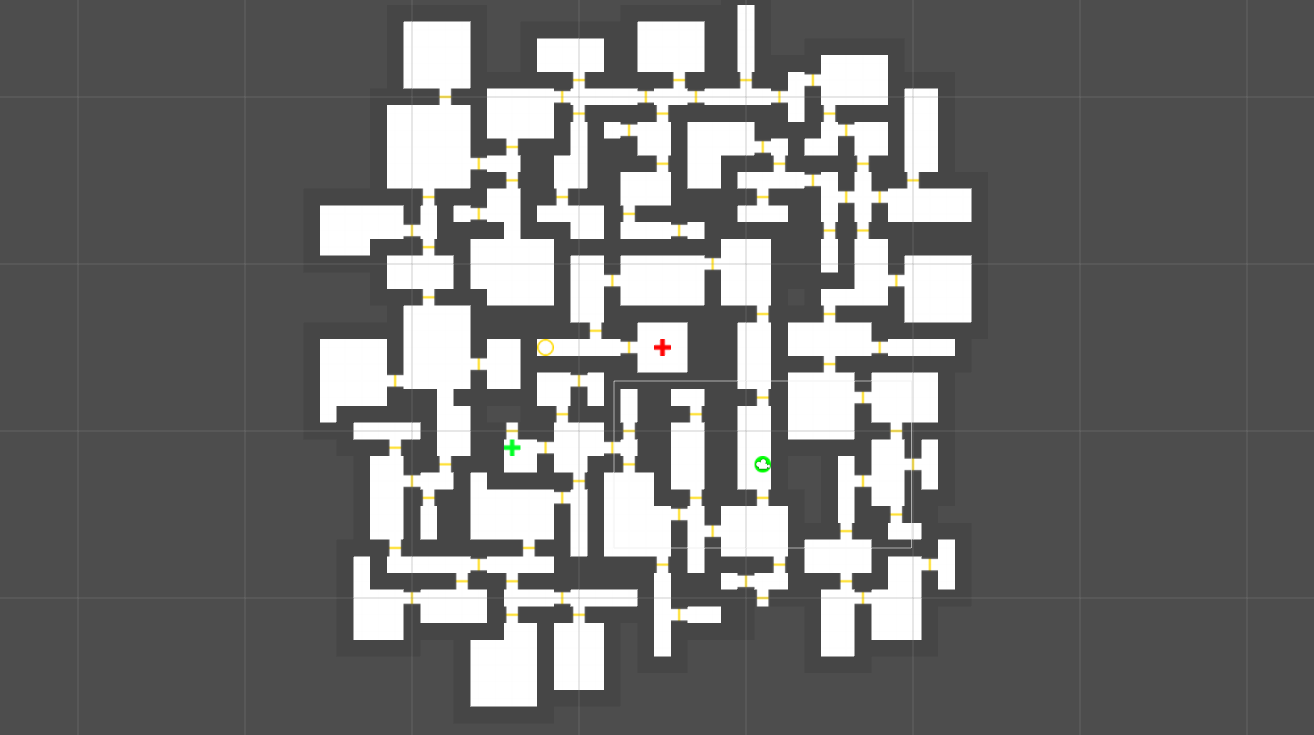
\includegraphics[width = \columnwidth ]{BigDungeon2.png}
	\caption{On this picture, you see the simple interface for selecting adventure mode or not.}
	\label{fig:behavTree}
\end{figure}
As you can see from the last picture, all the walls are closed off, and the player has explored the entire dungeon. The bugs with doors overlapping were fixed so that one door might be removed if the player chooses to go a different direction. This also only amplifies the feeling of adventure and choice/change that we wanted our game to have.

- Issues
* Misplacement of doors
* Overlapping of walls
* Too little time
\section{Discussion}
% conference papers do not normally have an appendix
«What are the strengths and shortcomings of your method? 
Why did you choose method X instead of Y? 
How well would it generalize to other game genres? 
How would you develop it further, if you had time?»



Further development: 
NPC spawning. 
NPC types, groups, interaction.
Better connections between doors/rooms/walls
Dungeon size reconfiguration


% use section* for acknowledgment
\ifCLASSOPTIONcompsoc
  % The Computer Society usually uses the plural form
  \section*{Acknowledgments}
\else
  % regular IEEE prefers the singular form
  \section*{Acknowledgment}
\fi



% trigger a \newpage just before the given reference
% number - used to balance the columns on the last page
% adjust value as needed - may need to be readjusted if
% the document is modified later
%\IEEEtriggeratref{8}
% The "triggered" command can be changed if desired:
%\IEEEtriggercmd{\enlargethispage{-5in}}

% references section

% can use a bibliography generated by BibTeX as a .bbl file
% BibTeX documentation can be easily obtained at:
% http://www.ctan.org/tex-archive/biblio/bibtex/contrib/doc/
% The IEEEtran BibTeX style support page is at:
% http://www.michaelshell.org/tex/ieeetran/bibtex/
%\bibliographystyle{IEEEtran}
% argument is your BibTeX string definitions and bibliography database(s)
%\bibliography{IEEEabrv,../bib/paper}
%
% <OR> manually copy in the resultant .bbl file
% set second argument of \begin to the number of references
% (used to reserve space for the reference number labels box)
\begin{thebibliography}{1}

\bibitem{IEEEhowto:kopka}
H.~Kopka and P.~W. Daly, \emph{A Guide to \LaTeX}, 3rd~ed.\hskip 1em plus
  0.5em minus 0.4em\relax Harlow, England: Addison-Wesley, 1999.
\bibitem{SpaceHulkvid}
Full Control and Games workshop, http://www.spacehulk-game.com/, Last visit: 13-12-2015
\bibitem{SpaceHulkBoard}
Games workshop, http://www.games-workshop.com/en-AU/Space-Hulk, Last visit: 13-12-2015
\bibitem{Diablo2}
Blizzard Entertainment, http://eu.blizzard.com/en-gb/games/d2/, Last visit: 13-12-2015
\end{thebibliography}

\end{document}


